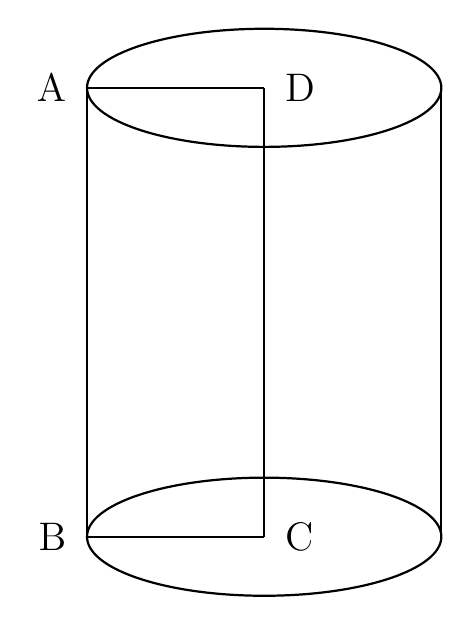
\begin{tikzpicture}[scale=1.5]
    % --- Definitions for Proportions ---
    \def\radius{1.5}    % Horizontal radius of the cylinder
    \def\vrad{0.5}      % Vertical radius (flatness) of the ellipses
    \def\height{3.8}    % Height of the cylinder

    % --- Coordinates ---
    \coordinate (C) at (0,0);           % Bottom Center
    \coordinate (D) at (0,\height);     % Top Center
    \coordinate (B) at (-\radius,0);    % Bottom Left
    \coordinate (A) at (-\radius,\height); % Top Left
    \coordinate (RightBot) at (\radius,0); % Bottom Right
    \coordinate (RightTop) at (\radius,\height); % Top Right

    % --- Drawing the Cylinder ---
    
    % 1. Bottom Ellipse (Full ellipse as shown in image)
    \draw[thick] (C) ellipse ({\radius} and {\vrad});
    
    % 2. Top Ellipse
    \draw[thick] (D) ellipse ({\radius} and {\vrad});
    
    % 3. Vertical Sides
    \draw[thick] (B) -- (A);           % Left side
    \draw[thick] (RightBot) -- (RightTop); % Right side

    % --- Drawing the Inner Rectangle (Generator lines) ---
    % Lines connecting the center axis to the edge
    \draw[thick] (A) -- (D); % Top radius
    \draw[thick] (B) -- (C); % Bottom radius
    \draw[thick] (C) -- (D); % Central axis

    % --- Labels ---
    % Positioned with offsets to match the reference image
    \node[left=4pt] at (A) {\Large A};
    \node[left=4pt] at (B) {\Large B};
    \node[right=4pt] at (C) {\Large C};
    \node[right=4pt] at (D) {\Large D};

\end{tikzpicture}